%  $Id: ManuelFR_v1.1.tex,v 1.3 2006/06/13 10:22:59 petiteau Exp $
\documentclass[a4paper,english,12pt]{article} 
\textwidth 16cm 
\textheight 21.cm 
\topmargin 1.5cm 
\oddsidemargin 0pt 
\evensidemargin 0pt 
\usepackage{graphicx} 
\usepackage{natbib} 
\usepackage{color} 
\usepackage{amsmath}
\usepackage{epstopdf} 
\pagestyle{headings} 

%\usepackage{pstopdf}
\pagestyle{headings}


\begin{document}
\title{
\Huge \bf LISACode \\ \Large version 1.4\\ \huge A scientific simulator of LISA \\ User's guide}
\author{\Large \bf LISA France}
\date{\today}
\maketitle

\setcounter{page}{1}

\newpage

$ $
%Redefinition de la hauteur de la page et du haut%
\textheight 23.cm
\topmargin 0.2cm


\setcounter{page}{1}

\tableofcontents
\newpage



\definecolor{pink}{rgb}{0.55,0,0.52}


\newpage

%*****************
% * Introduction  *
%*****************

\section{Introduction}
\label{SIntro}
This document provides a description of the LISACode software. LISACode simulates the LISA  gravitational wave (GW) detector (ref) . It does not aim to simulate in detail the detector itself but rather it makes use of the response function of its main components, particularly in the way they will affect the noise level of the detector response. It also includes an implementation of the TDI (Time Delay Interferometry) technique which allows to suppress the noise level of the lasers. \\

The main inputs and outputs of LISACode are time-dependent sequences that will describe, for input and as a function of time, the GW strain  and for output, and also as a function of time, the phasemeters response or their treatment via various TDI combination, in order to remove the laser noise level. \\

A number of  elementary GW signals can be defined , but also it's possible to use the code in conjunction with more sophisticated GW simulators via intermediate data files. \\

The main outputs of the code will be a number of time dependent data signals which will be produced either directly from the phasemeters or from a TDI treatment of these. \\

This document describes, in section II, the structure of the code. Section III will explain how the code can be installed on a variety of platforms. Section IV describes the use of LISACode The section V describes the configuration file, a list of the main parameters that controls its operations and output.  \\

More scientific information on LISACode are available in article of A.Petiteau \cite{LISACode}.

\section{A description of the Code}
\label{SCode}
This software is written in C++ for use the modularity of the object programming. The main structure of LISACode is shown in the figure \ref{Struct_LISACode}. This structure maps the main components of the LISA detector as well as its physical inputs.

\begin{figure}[!h]
\centering 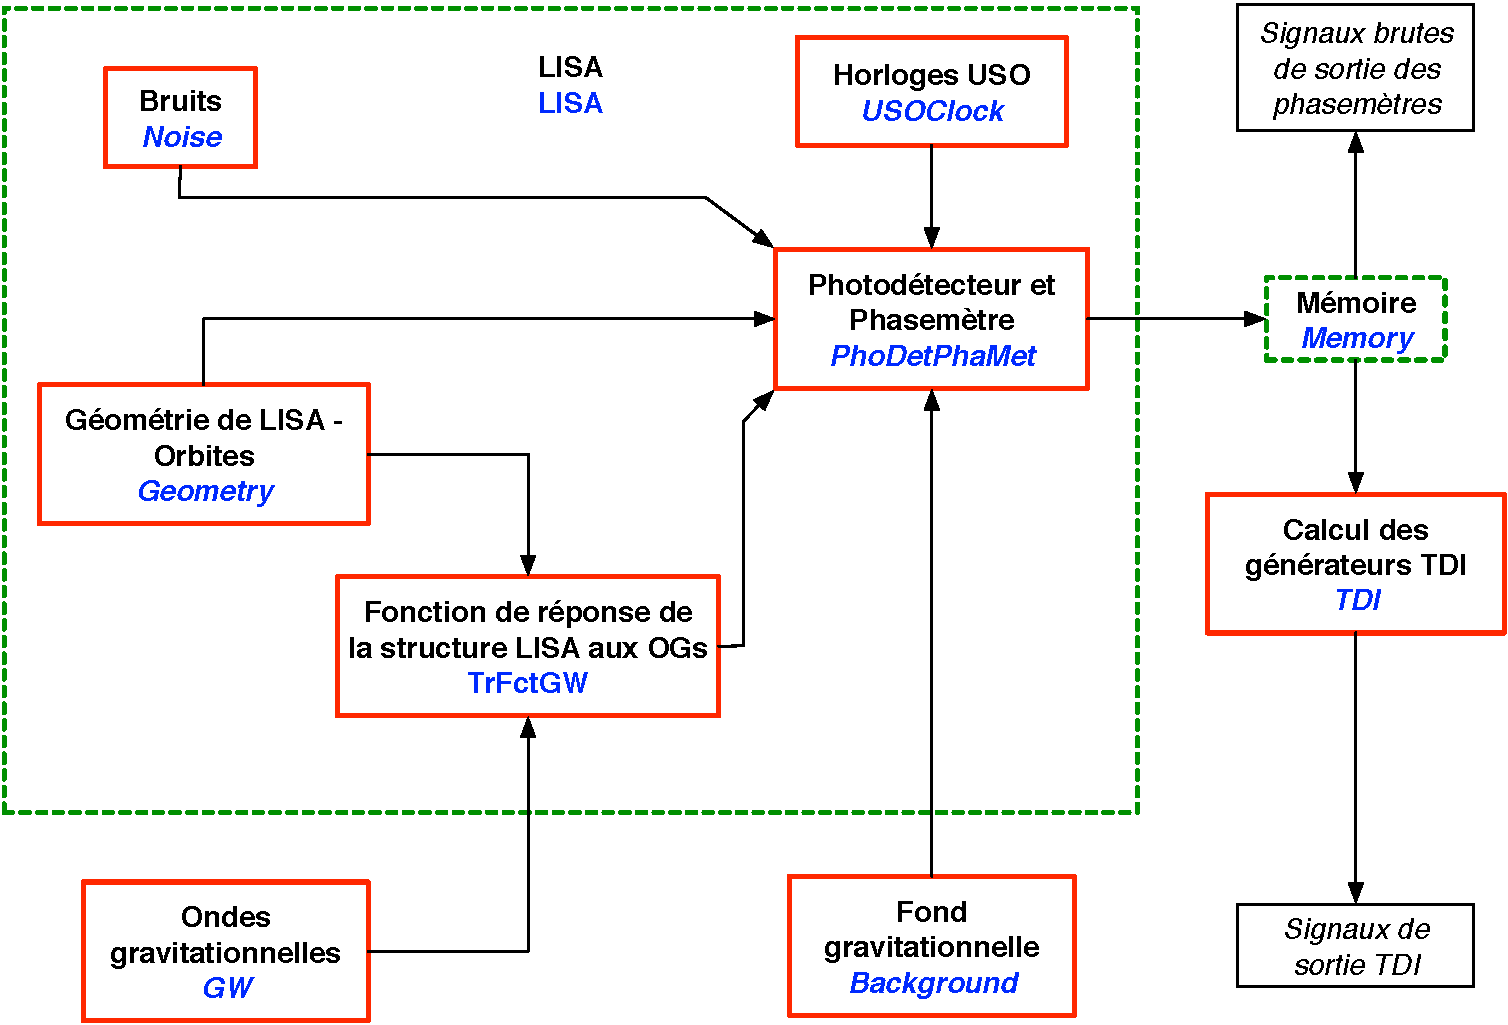
\includegraphics[width=14cm]{Figures/Structure.pdf}
\caption{\small Structure of simulator LISACode. The \textcolor{red}{red} boxes represent the main modules and the \textcolor{green}{green} boxes the interface modules. The module's generic name is in \textcolor{blue}{blue}.\small} 
\label{Struct_LISACode}
\end{figure}

There are 9 libraries : 
\begin{itemize}
\item {\em Outils\_Maths} : Objects use like tools the others modules : vector, filters, ...
\item {\em Ondes\_Gravit} : Model \textbf{gravitational waves (GW)}.
\item {\em Orbitographie} : Model spacecraft orbits.
\item {\em Bruits} : Model noises.
\item {\em USO\_Temps} : Model ultra-stable oscillators.
\item {\em Memoire} : Manage memories for output data of each spacecraft.
\item {\em Input\_Data} : Read configuration of simulator.
\item {\em Detecteur} : Model LISA detector : Arm response at gravitational waves, phasemeters, general running.
\item {\em TDI} : Apply TDI generator.
\end{itemize}

The figure \ref{Org_LISACode} shows the organisation of the libraries used by LISACode. \\

\begin{figure}[!h]
\centering 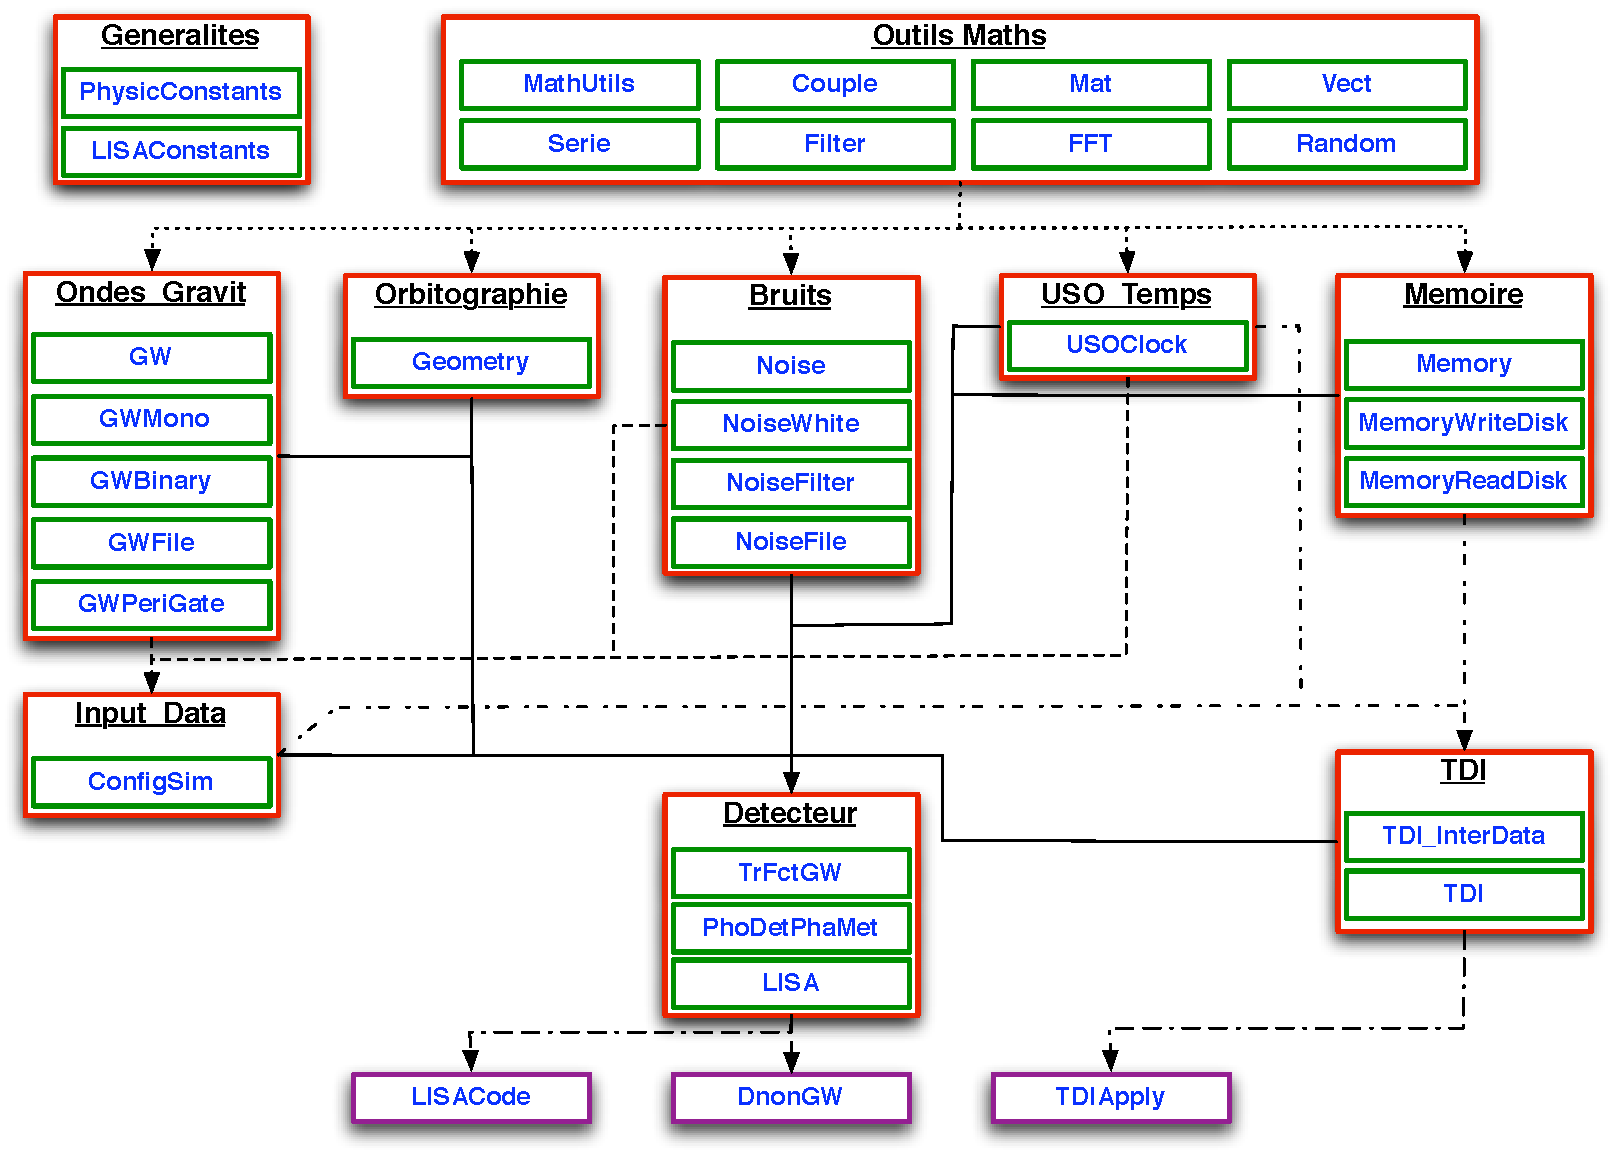
\includegraphics[width=15cm]{Figures/OrgPackage.pdf}
\caption{\small Organisation and dependency  for simulator's libraries. The  \textcolor{green}{green} boxes represent objects, the \textcolor{red}{red} boxes the libraries and the \textcolor{pink}{pink} boxes the executables.\small} 
\label{Org_LISACode}
\end{figure}

The first input is the GW itself. It can be defined either internally through some models which produce signals from any monochromatic sources, binary system with fixed frequency or binary system computed in Post-Newtonian approximation (1 or 2.5 PN). The GW can also be inputted via a GW time sequence as may be produced by more sophisticated simulator codes.  \\

The orbits of LISA are generated internally via the code. They correspond to realistic orbits that contain both the breathing and rotation modes of LISA as a function of its rotation around the sun. The parameters of these orbits can be adjusted in order to modify the average distance between the satellites (nominally $5 \times 10^{9} \; m$) or be defined in such a way as to keep LISA at a fix and given location. The initial location of the orbits can also be defined at input.\\

An important ingredient of the LISA response and hence of the codes are the noise inputs of different nature. These include the optical noise due to shot noise and related factors as described in table \ref{table_error}. The inertial mass and the laser noises can also be defined at input. Normally, these noise are defined as bandwidth limited white noise but different shapes of noise can be used.

\begin{table}[htdp] 
\caption{Error allocation budget based on Table 4.1 of  \cite{PrePhaseAReport}.  
The fourth column gives the default error included in LISACode. These values can be  
modified by the user. The frequency dependence of these noises is discussed in \ref{SSSConfigGW}} 
\begin{center} 
\small
\begin{tabular}{|c|c|c|c|c|} 
\hline 
Error source & Error & LISACode & LISACode input ($\delta \nu \over \nu $ unit)  \\ 
\hline 
\multicolumn{4}{|c|}{Measurement Noise}  \\ 
\hline 
Detector shot noise&$11\times 10^{-12} {\rm m.{Hz}^{-{1 \over 2}}}$&$11$ & \footnotesize$ 2.3 \times 10^{-19}\left(f\over 1 Hz \right) \left(L \over 5 \times 10^{9}{\rm m} \right) \sqrt{1 {\rm  W}\over P }.{Hz}^{-{1 \over 2}} $\small \\ 
\hline 
USO & $5 \times10^{-12} {\rm m.{Hz}^{-{1 \over 2}}}$& &  \\  
\cline{1-2} 
Residual laser phase noise&$5 \times 10^{-12} {\rm m.{Hz}^{-{1 \over 2}}}$& &  \\ 
\cline{1-2} 
Laser beam-pointing &$10 \times10^{-12} {\rm m.{Hz}^{-{1 \over 2}}}$& $16.5$ & $3.49 \times 10^{-19} \left(f\over 1 Hz \right).{Hz}^{-{1 \over 2}}$\\ 
instability& & &  \\ 
\cline{1-2} 
Laser phase measurement &$5\times10^{-12} {\rm m.{Hz}^{-{1 \over 2}}}$& &  \\ 
and offset lock& & &  \\ 
\cline{1-2} 
Scattered-light effects&$5\times10^{-12} {\rm m.{Hz}^{-{1 \over 2}}}$& &  \\ 
\cline{1-2} 
Other substancial effects&$8.5\times10^{-12} {\rm m.{Hz}^{-{1 \over 2}}}$& & \\ 
\hline 
\multicolumn{4}{|c|}{Acceleration Noise}  \\ 
\hline 
Inertial Mass noise & $3 \times10^{-15}{\rm m.s^{-2}.{Hz}^{-{1 \over 2}}}$& $3 $ & $1.59 \times 10^{-24} \left( 1 Hz \over f\right).{Hz}^{-{1 \over 2}}$\\ 
\hline 
\end{tabular} 
\end{center} 
%\label{default} 
\label{table_error} 
\end{table}% 
\normalsize

Using the orbits, the response of LISA to the GW will be calculated and a relative frequency fluctuation (unit in $\Delta \nu \over \nu$) will be inputted to the Phasemeter Module. These will be combined with the different noise contribution to produce the primary phasemeter output signal which then will be processed through a elliptic filtering module. This filter is low-pass filter which cuts the frequency at half of measurement frequency for cancel the spectrum aliased. In standard operation, the primary signal will be produced at a 0.5 Hz signal and outputted, after filtering, at a 1 Hz rate. \\

This signal can be saved on a disk file and/or processed by a TDI module using a variety of TDI combinations that are defined at input. A  detailed description of TDI combination can be found in ref \cite{TDIVinet} and in ref \cite{TDITinto}. \\

The above description of the code provides only a brief summary of its capabilities. 
%The next section will provide a (non-exhaustive) list of the parameters that can be used to control the input, the processing and the output of the code and will therefore give a more complete idea of its possibilities.

\newpage

%%%%%%%%%%%
%  INSTALLATION  %
%%%%%%%%%%%
\section{Installation}
\label{SInstall}
\subsection{System requirements}
\label{SSSystReq}
This software can be installed on UNIX system which have a standard C and C++ compiler.\\
There is also a Windows executable (tested only for Windows XP).\\ 

%
%   UNIX
%
\subsection{For Unix, Linux, Mac OS X}
\label{SSInstallUNIX}
\subsubsection{Install}
\label{SSSInstallUNIX}
The installation is the same as a standard UNIX software. The following procedure describes the installation steps : 
\begin{enumerate}
\item Download the package lisacode-1.3.tar.gz\\ (on the web : http://www.apc.univ-paris7.fr/Downloads/lisa/LISACode/ )\\ and move the package in the directory ({\it MyDirectory} in the example) where you want to install LISACode.
\item Uncompress the package : \\
\hphantom{aaaaa}\texttt{tar xvzf lisacode-1.3.tar.gz }\\
\item Go in the {\it LISA\_Sim\_Tdi} directory :\\
\hphantom{aaaaa}\texttt{cd MyDirectory/lisacode-1.3 }\\
\item Execute configuration scipt, {\it configure}, for make the {\it makefile} : \\
\hphantom{aaaaa}\texttt{./configure}\\
It's possible to add  compilation options and the directory where the executable will be installed (see the part \ref{SSSInstallConfig} or the file {\it INSTALL} for more technicalities on this two points).
\item Execute the {\it makefile} for compile the code : \\
\hphantom{aaaaa}\texttt{make}
\item If you want to install the simulator with your computer's executables or in specified directory, use the command : \\
\hphantom{aaaaa}\texttt{make install}
\end{enumerate}

If the software has been installed correctly, there are 3 main executables in the directory {\it MyDirectory/lisacode-1.3/Main/Test}. The 3 main executables are :
\begin{itemize}
\item {\em LISACode} : The main simulator executable which models gravitational wave, processes them in LISA detector and apply TDI on the output data.
\item {\em DnonGW} : Executable which gives relative frequency fluctuations on the beams made by gravitational waves.
\item {\em TDIApply} : Apply TDI generators on phasemeters output data.
\end{itemize}
If you use {\it make install} for compile, the 3 executables are also in the directory {\it bin} located with your computer's executable or in specified directory {\it MyExe/bin}. There are also many test executable in this directory.\\

For more useful, copy the executables in your work directory (the directory where you want to make LISA simulation).


\subsubsection{Installation configuration}
\label{SSSInstallConfig}
Many installation options are detailed in the file {\it INSTALL} located in {\it MyDirectory/lisacode-1.3}.\\

The compilation options should be specified with the configuration. After \texttt{./configure}, enter \texttt{CXXFLAGS=} followed by compilation options. For example, to optimise the compilation on PowerPCG5, the option is {\it -O3 -fast} therefore the configuration command is : \\
\hphantom{aaaaa}\texttt{./configure CXXFLAGS="-O3 -fast -Wno-deprecated"} \\ 

It also possible to specify the path of the directory where the executables will be installed, with the command \texttt{make install}. Enter \texttt{--prefix=} followed by the directory path. For example, the configuration command may be used on PowerPCG5 with exectables in the directory {\it MyExe} is : \\
\hphantom{aaaaa}\texttt{./configure CXXFLAGS="-O3 -fast -Wno-deprecated" --prefix="MyExe"} \\

\subsubsection{Running test}
\label{SSSTestFonctUNIX}
For test the running of LISACode, use configuration file ({\it ConfigRefBase}) with the followed instructions : \\
\begin{enumerate}
%\item Copy the file {\it ConfigRefBase} located in {\it MyDirectory/lisacode-1.3}, in any worked directory.
\item Go in LISACode directory {\it MyDirectory/lisacode-1.3}.
\item Launch the simulator : Execute {\it LISACode} followed by the name of the configuration file  {\it ConfigRefBase} then  "123456" (seed of random generator). \\
If you use {\it make} for configuration, enter : \\
\hphantom{aaaaa}\texttt{Main/bin/LISACode ConfigRefBase 123456} \\
Else, if you use {\it make install} for configuration, enter : \\
\hphantom{aaaaa}\texttt{MyExe/LISACode ConfigRefBase 123456}
\end{enumerate}
The software run during about 10 secondes or 3 minutes , for make 10 000 s of simulation. The final display is : \\
\texttt{...}\\
\texttt{10000 s     \#0100 \%} \\
\hphantom{aaaaa}\texttt{ X = 9.41546278836602e-19}\\
\hphantom{aaaaa}\texttt{ Y = 9.73859038667986e-19}\\
\hphantom{aaaaa}\texttt{ Z = 9.28457478808582e-19}\\
\hphantom{aaaaa}\texttt{ AlphaMan = 6.41358600758029e-19}\\
\hphantom{aaaaa}\texttt{ Beta = 6.48014274920517e-19}\\
\hphantom{aaaaa}\texttt{  X2s1 = 8.97752170019294e-19}\\
\hphantom{aaaaa}\texttt{ X2s2 = 9.41500592699302e-19}\\
\hphantom{aaaaa}\texttt{ X2s3 = 8.16992767767782e-19}\\
\hphantom{aaaaa}\texttt{ P1 = 4.98540196959974e-19}\\
\hphantom{aaaaa}\texttt{ Zeta1 = 7.07135169910109e-20}\\
\texttt{Final time : 10001 s}\\
\texttt{End}\\


%
%   Windows
%
\subsection{Sous Windows}
\label{SWindows}
There is a LISACode executable for Windows which is tested on Windows XP.
\subsubsection{Install}
\label{SSInstallWindows}
There isn''t really install ; just download the package {\it LISACode\_1\_3\_for\_Windows.zip}  at : \\
 {\it http://www.apc.univ-paris7.fr/Downloads/lisa/LISACode/version-1.3/}.\\
Uncompress the package and run  LISACode.exe.
\subsubsection{Test}
\label{SSSTestFonctWindows}
It's possible to test the running of LISACode with the configuration file ({\it ConfigRefBase}) which is located in the same directory than the executable. Follow this instructions : \\
\begin{enumerate}
\item Open MS-DOS terminal and go to the executable where there are LISACode executable and run the configuration file {\it ConfigRefBase} (\texttt{cd ...} ).
\item Run the simulator : {\it LISACode} followed by the name of the configuration file  ({\it ConfigRefBase}) and "123456" (seed of random generator) . \\
\hphantom{aaaaa}\texttt{LISACode.exe ConfigRefBase 123456}
\end{enumerate}
The result is the same than~\ref{SSSTestFonctUNIX}.


\newpage

%%%%%%%%%%%
%  USE LISACODE  %
%%%%%%%%%%%
\section{Use LISACode}
\label{SUse}
\subsection{Ex\'ecution of simulator and the two annexe softwares}
\label{SSExecution}
The main software which make all the simulation (from gravitational waves to TDI) is called LISACode.
For configure the simulation the software read informations in the configuration file. This configuration file may be two type : ASCII or XML. The technicalities of this configuration file is gave in the part \ref{SSConfigFile}. The path of the output files is in the configuration file. For launch a simulation, enter LISACode executable path followed by the configuration file path : \\
\hphantom{aaa}\texttt{./LISACode configuration\_file}\\
{\it(if the LISACode executable is in the work directory)}\\
\hphantom{aaa}ou\\
\hphantom{aaa}\texttt{MyExe/LISACode configuration\_file}\\
{\it(if the LISACode executable isn't in the work directory)}\\

There are two others executables which also read information on configuration file. They make only one parts of the simulation : \\
\begin{itemize}
\item {\it \bf DnonGW} : This program computes the relative frequency fluctuations on the laser beam which arrive on each phasemeter with only the gravitational response.  There are 3 output files which have always the same name : \\
\begin{itemize}
\item {\it DnGW\_GW.txt} : Time evolution of gravitational waves' polarisation components $h_+$ and $h_\times$.
\item {\it DnGW\_Position.txt} : Time evolution of spacecrafts' ecliptic coordinates.
\item {\it DnGW\_TDelay.txt} : Time evolution of flightpath between spacecraft.
\item {\it DnGW\_SigFctTrGW.txt} : Time evolution of relative frequency fluctuation for external laser beams which arrive on each spacecraft.
\end{itemize}
The time parameters are specified in configuration file.\\

\item {\it \bf TDIApply} : This program apply TDI generator specified in configuration file, on phasemeter raw data read in files specified in configuration file. The output contains time evolution for each TDI generator. The name of this ouput file is specified in configuration file.
\end{itemize}

%%%%%%%%%%%%%%%
%  CONFIGURATION FILE  %
%%%%%%%%%%%%%%%
\section{Configuration file}
\label{SConfigFile}

% Generalites  
%%%%%%%%
\subsection{Generalities}
\label{SSConfGen}
This file contains all the information for simulator configuration. There two types of possible file : ASCII or XML.  The XML file can be made with a graphical interface software : {\it LISA\_AutoGUI.jar}. The tables \ref{table_paramTime} , \ref{table_paramPrecisionTDI}, \ref{table_paramOrbits}, \ref{table_paramDetector}, \ref{table_paramRecord}, \ref{table_paramGW}, \ref{table_paramNoise} , \ref{table_paramUSO} and \ref{table_paramTDI}    lists the parameters.

\begin{table}[p] 
\caption{List of parameters used to configure a simulation whose type is \textbf{Time}. }
\begin{center} 
\begin{tabular}{|p{3.cm}|p{8.cm}|c|p{1.in}|} 
\hline 
Name & Explanation & Unit & Standard Value  \\ 
\hline 
 StepPhysic & Time step use for model the continuous process, prior to filtering. & second & 0.5 \\ 
\hline 
 StepMeasure & Time step of output file of Phasemeter signal, after filtering. & second & 1 \\ 
\hline 
 Max & Total duration of calculation. & second & from second to years \\ 
\hline 
 DeltaTDIDelay & Possible error on the estimation of the delay. & second & from 0 to 1e-5 \\ 
\hline 
 StepDisplay & Time step of evolution display (for follow the simulation). & second & from 100 to 1e6 \\ 
\hline 
\end{tabular} 
\end{center} 
\label{table_paramTime} 
\end{table}

\begin{table}[p] 
\caption{List of parameters used to configure a simulation whose type is \textbf{PrecisionTDI}. }
\begin{center} 
\begin{tabular}{|c|p{8.cm}|c|c|} 
\hline 
Name & Explanation & Unit & Standard Value  \\ 
\hline
 Interpolation & Type of interpolation performed for TDI &  & LAG 20 \\ 
\hline 
 TDIDelayApprox & If ON, delays use in TDI are added else they are imbricated  & On/Off & Off \\ 
 \hline
\end{tabular} 
\end{center} 
\label{table_paramPrecisionTDI} 
\end{table}

\begin{table}[p] 
\caption{List of parameters used to configure a simulation whose type is \textbf{Orbits}. }
\begin{center} 
\begin{tabular}{|c|p{8.cm}|p{3.cm}|p{2.cm}|} 
\hline
Name & Explanation & Unit & Standard Value  \\ 
\hline
 Armlength & Average armlength between LISA satellites & meters & 5e9 \\ 
\hline 
 StartTime & Start time which defines the LISA position on the orbits at beginning of calculation.  & seconds (From 0 to year) & 0 \\ 
\hline 
 InitialRotation & Initial phase of LISA triangle configuration (0 : spacecraft 1 at bottom) & radians & 0 \\ 
\hline 
 Move & If On LISA spacecraft move else LISA spacecraft are fixed.  & On/Off & On \\ 
\hline 
 Order & Order of flightpath calculation : 0 - time computed as from spacecraft positions ,1 - Sagnac effect , 2 - General  Relativity effects.  & 0 / 1 / 2 & 2 \\ 
\hline 
\end{tabular} 
\end{center} 
\label{table_paramOrbits} 
\end{table}

\begin{table}[p] 
\caption{List of parameters used to configure a simulation whose type is \textbf{Detector}. }
\begin{center} 
\begin{tabular}{|p{3.cm}|p{1.in}|p{6.cm}|p{2.cm}|p{2.cm}|} 
\hline 
 \multicolumn{2}{|c|}{Name} & Explanation & Unit & Standard Value  \\ 
\hline
 \multicolumn{2}{|c|}{LaserPower} & Defines the Laser power.  & Watt & 1 \\ 
\hline 
\multicolumn{2}{|c|}{PhaMetFilter} & Activates or de-activates Phasemeter Filter.  & On/Off & On \\ 
\hline 
 PhaMetFilter-Parameters  &  attenuation &  Filter attenuation & dB & 180 \\
 \hline
 PhaMetFilter-Parameters  &  oscillation &  Filter oscillations in bandwidth & dB & 0.1 \\ 
 \hline
 PhaMetFilter-Parameters  &  FactFmes-ForHighFreq & Factor for high transition frequency ( high transition frequency over measurement frequency ) &  & 0.1 \\ 
 \hline
 PhaMetFilter-Parameters  & FactFmes-ForLowFreq & Factor for  low transition frequency ( low transition frequency over measurement frequency ) &  & 0.3 \\ 
 \hline
\end{tabular} 
\end{center} 
\label{table_paramDetector} 
\end{table}

\begin{table}[p] 
\caption{List of parameters used to configure a simulation whose type is  \textbf{Records}. }
\begin{center} 
\begin{tabular}{|c|p{8.cm}|c|} 
\hline 
 Name & Explanation &  Standard Value  \\ 
\hline
 SignalSC 1& Defines output file name which contains spacecraft 1 phasemeters' raw data.  &  SC1.txt \\ 
\hline
 SignalSC 2& Defines output file name which contains spacecraft 2 phasemeters' raw data.  &  SC2.txt \\
\hline
SignalSC 3& Defines output file name which contains spacecraft 3 phasemeters' raw data.  &  SC3.txt \\ 
\hline
Delay & Defines output file name which contains 6 flightpath data in seconds.  &  Delay.txt \\ 
\hline
Position & Defines output file name which contains ecliptic coordinates of the 3 spacecrafts in meters.  &  Delay.txt \\ 
\hline
TDI & Defines output file name which contains data of specified TDI generators.  &  TDI.txt \\ 
\hline 
\end{tabular} 
\end{center} 
\label{table_paramRecord} 
\end{table}

\begin{table}[p] 
\caption{List of parameters used to configure a simulation whose type is  \textbf{GW} (see figure \ref{GWParameters} ) \textbf{Mono} defines a monochromatic wave, \textbf{Binary} defines a binary system with fixed frequency and \textbf{PostNewtonBinary} defines a binary system which is computed in Post-Newtonian approximation. }
\begin{center} 
\begin{tabular}{|p{33.mm}|p{15.mm}|p{65mm}|p{2.cm}|p{18.mm}|} 
\hline 
\textbf{GW Type} & \textbf{Name} & \textbf{Explanation} & \textbf{Unit} & \textbf{Standard Value}  \\ 
\hline
All & Bet & Ecliptic latitude (declination) of source direction (from Sun to source) & degrees & from -90 to 90 \\
\hline
All & Lam & Ecliptic longitude of source direction (from Sun to source) & degrees & from 0 to 360 \\
\hline
All & Psi & Polarisation of the source : angle between the observational reference frame and the canonical reference frame & degrees & from 0 to 360  \\
\hline
\hline
Mono & f & Frequency of the source & Hertz &   \\
\hline
Mono & hp & Amplitude of $+$ component. & none &1e-21  \\
\hline
Mono & hc & Amplitude of $\times$ component. & none &1e-21  \\
\hline
Mono & Phi0hp & Initial phase of $+$ component. & radians & 0 to $2 \pi$  \\
\hline
Mono & Phi0hc & Initial phase of $\times$ component. & radians & 0 to $2 \pi$  \\
\hline
\hline
Binary & M1 & Mass of first object & solar mass&   \\
\hline
Binary & M2 &  Mass of second object & solar mass &  \\
\hline
Binary & forb & Orbital frequency of binary system. & Hertz &  \\
\hline
Binary & inc & Inclination : angle between angular momentum and source's direction & degrees & from -90 to 90 \\
\hline
Binary & phi0 & Initial phase of binary system. & radians & 0 to $2 \pi$  \\
\hline
Binary & r & Distance between the observator and the source. & KiloParsec &  \\
\hline
PostNewtonBinary & M1 & Mass of first object & solar mass&   \\
\hline
PostNewtonBinary & M2 &  Mass of second object & solar mass &  \\
\hline
PostNewtonBinary & tcoal & Coalescence time (start at 0 at the beginning of the simulation). & seconds &  \\
\hline
PostNewtonBinary & inc & Inclination : angle between angular momentum and source's direction & degrees & from -90 to 90 \\
\hline
PostNewtonBinary & phase & Initial phase of binary system. & radians & 0 to $2 \pi$  \\
\hline
PostNewtonBinary & r & Distance between the observator and the source. & KiloParsec &  \\
\hline
\hline
PostNewtonBinary & type & Type of Post-Newtonian calculation : 1 for 1 PN and 2 for 2.5 PN. & 1 / 2 & 2 \\
\hline
PostNewtonBinary & omega0 & Arbitrary Post-Newtonian phase. & degrees & 1 \\
\hline
PostNewtonBinary & taud0 & Post-Newtonian phase on the detector. &  & 10  \\
\hline
PostNewtonBinary & gw & Post-Newtonian factor. &  & 1 \\
\hline
\end{tabular} 
\end{center} 
\label{table_paramGW} 
\end{table}

\begin{figure}[p] 
\centering 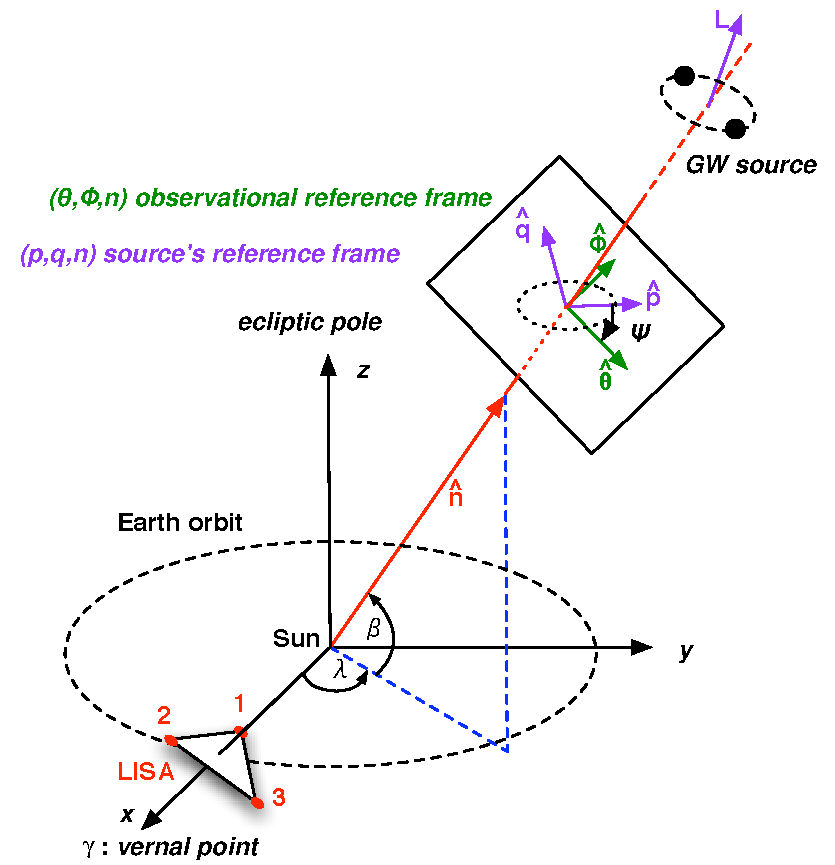
\includegraphics[width=10cm]{Figures/GWParameters.pdf} 
\caption{\small Schematic description of GW parameters and reference frames.  
The direction fo the source is located by the declination $\beta$ and the ecliptic  
longitude $\lambda$. ($ \widehat{\theta}$, $ \widehat{\phi}$, $\widehat{n}$)  is the  
observational reference frame , i.e. the frame  constructed from the direction of the source.  
In this frame $ \widehat{\theta}$ is on the meridian.   
($ \widehat{p}$, $ \widehat{q}$, $\widehat{n}$) is the canonical reference frame .  
$\psi$ is the polarization angle, i. e. the angle between the canonical reference frame   
and the observational reference frame.} 
\label{GWParameters} 
\end{figure} 

\begin{table}[p] 
\caption{List of parameters used to configure a simulation whose type is  \textbf{Noise} (see figure \ref{SchBOSC1} for localization). }
\begin{center} 
\begin{tabular}{|p{22.mm}|p{20.mm}|p{65mm}|p{3.cm}|p{18.mm}|} 
\hline 
\textbf{Parameter type} & \textbf{Name} & \textbf{Explanation} & \textbf{Unit} & \textbf{Standard Value}  \\ 
\hline
Localization & Laser i j & \multicolumn{3}{|p{110.mm}|}{ Noise of the laser located in optical bench of the spacecraft i pointing towards the spacecraft i+1 if j = 0 and towards the spacecraft i-1 if j = 1. } \\
\hline
Localization & Mass i j & \multicolumn{3}{|p{110.mm}|}{ Noise of the inertial mass located in optical bench i j (i.e. laser i j optical bench). } \\
\hline
Localization & Shot i j & \multicolumn{3}{|p{110.mm}|}{ Shot noise of the phasemeters  which measure the interference between the beam from the distant spacecraft and the beam of  the local optical bench i j (i.e. laser i j optical bench). } \\
\hline
Localization & OOPN i j & \multicolumn{3}{|p{110.mm}|}{ Others optical path noise located in optical bench i j (i.e. laser i j optical bench). } \\
\hline
Type & White  & White noise at specified level. & ${\Delta \nu \over \nu} . Hz^{-1/2} $ unit & 1e-13 \\
\hline
Type & Filter\_1of  & Filter noise corresponds to function 1/f at specified level. & ${\Delta \nu \over \nu} . Hz^{-1/2} $ unit & 1.59e-24 \\
\hline
Type & Filter\_f  & Filter noise corresponds to function f at specified level. & ${\Delta \nu \over \nu} . Hz^{-1/2} $ unit & 3.49e-19 \\
\hline
Type & Filter\_fLosP  & Filter noise corresponds to function f at specified level proportional to the armlength and inversely proportional to the root square of power. & ${\Delta \nu \over \nu} . Hz^{-1/2} $ unit & 2.30e-19 \\
\hline
Type & FilterCoef  & Filter noise where the filter coefficient are specified explicitly : & &  \\
 & - alpha & Recursive coefficient of filter & &  \\
 & - beta & Direct coefficient of filter & &  \\
 & - stabilization & Number of data for filter stabilisation & steps &  10000 \\ 
\hline
\end{tabular} 
\end{center} 
\label{table_paramNoise} 
\end{table}

\begin{figure}[p] 
\centering 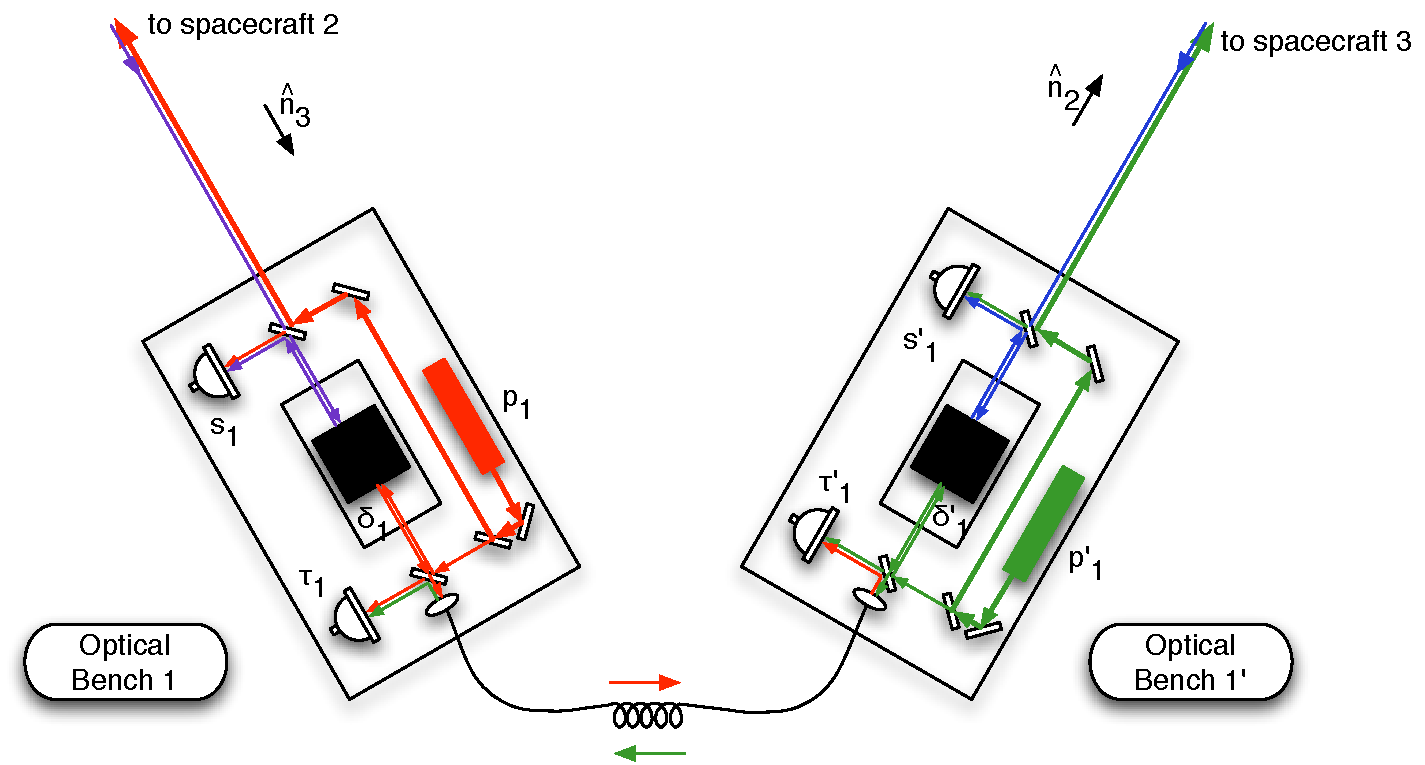
\includegraphics[width=10cm]{Figures/SchBOSC1.pdf} 
\caption{\small Schematic representation of the two optical benches of spacecraft 1.  
$s_{i}$ and $s'_{i}$ are the phasemeters which measure the interference between the  
beam from the distant spacecraft and the beam of  the local optical bench, i.e.  
containing the phasemeter. $\tau_{i}$ and $\tau'_{i}$ are the phasemeters which measure  
the interference between the beam from the other optical bench in the same spacecraft  
and the beam of the optical bench which contains the phasemeter. $p$ is the laser and   
$\delta$ is the inertial mass(form \cite{TDITinto}).}   
\label{SchBOSC1} 
\end{figure}

\begin{table}[p] 
\caption{List of parameters used to configure a simulation whose type is  \textbf{USO}. There is one USO by spacecraft specified by \textbf{SC} followed by the spacecraft number}
\begin{center} 
\begin{tabular}{|c|p{8.cm}|p{3.cm}|p{2.cm}|} 
\hline
Name & Explanation & Unit & Standard Value  \\ 
\hline
 offset & Offset of USO compared to current time & seconds & 0.006 \\ 
\hline
 derivs & Derive of USO compared to current time in second by seconds & seconds & 1e-7 \\ 
\hline
 noise & Gaussian noise of USO compared to current time  with specified $\sigma$& seconds & 1e-7 \\ 
\hline
\end{tabular} 
\end{center} 
\label{table_paramUSO} 
\end{table}

\begin{table}[p] 
\caption{List of parameters used to configure a simulation whose type is  \textbf{TDI}. (\textbf{SC} mean spacecraft)}
\begin{center} 
\begin{tabular}{|p{35.mm}|p{60.mm}|p{65.mm}|} 
\hline
Name & Explanation & Pack Value (in LISACode) \\ 
\hline
{\it Any name} & Any TDI generator & to be define after the name \\ 
\hline
X or Xf or X1s1 & Michelson first generation centred on SC1 & 1 , 35 , 364 , 3653 , -4 , -53 , -521 , -5235  \\ 
\hline
Y or Yf or X1s2 & Michelson first generation centred on SC2 & 2 , 16 , 145 , 1461 , -5 , -61 , -632 , -6316  \\ 
\hline
Z or Zf or X1s3 & Michelson first generation centred on SC3 & 3 , 24 , 256 , 2542 , -6 , -42 , -413 , -4124  \\ 
\hline
X2 or Xf2 or X2s1 & Michelson second generation centred on SC1 & 1 , 35 , 364 , 3653 , 36524 , 365253 , 3652521 , 36525235 ,  -4 , -53 , -521 , -5235 , -52361 , -523635 , -5236364 , -52363653  \\ 
\hline
Y2 or Yf2 or X2s2 & Michelson second generation centred on SC2 & 2 , 16 , 145 , 1461 , 14635 , 146361 , 1463632 , 14636316 , -5 , -61 , -632 , -6316 , -63142 , -631416 , -6314145 , -63141461  \\ 
\hline
Z2 or Zf2 or X2s3 & Michelson second generation centred on SC3 & 3 , 24 , 256 , 2542 , 25416 , 254142 , 2541413 , 25414124 , -6 , -42 , -413 , -4124 , -41253 , -412524 , -4125256 , -41252542  \\ 
\hline
Alpha or alpha & Basic generator first generation $\alpha$ & -1 , -32 ,  -133 , 4 , 455 , 56  \\ 
\hline
Beta or beta & Basic generator first generation $\beta$ & -121 , -2 , -13 , 64 , 5 , 566  \\ 
\hline
Gamma or gamma &Basic generator first generation $\gamma$ & -21 , -232 , -3 , 464 , 45 , 6  \\ 
\hline
P1 & Beacon generator with no beams received by SC1 & 25 , -63 , -22 , 66 , 642 , -216 , 1463 , -1425  \\ 
\hline
Q1 & Beacon generator with no beams received by SC2 & 36 , -41 , -33 , 44 , 453 , -324 , 2541 , -2536  \\ 
\hline
R1 & Beacon generator with no beams received by SC3 & 14 , -52 , -11 , 55 , 561 , -135 , 3652 , -3614  \\ 
\hline
E1 & Monitor generator with no beams emitted by SC1 & 542 , 56 , -316 , -32 , -144 , 141 , 4 , -1  \\ 
\hline
F1 & Monitor generator with no beams emitted by SC2 & 653 , 64 , -124 , -13 , -255 , 252 , 5 , -2  \\ 
\hline
G1 & Monitor generator with no beams emitted by SC3 & 461 , 45 , -235 , -21 , -366 , 363 , 6 , -3  \\ 
\hline
U1 & Relay generator with no beams from SC3 to SC1 and  from SC1 to SC2 & 145 , 1464 , -5 , -64 , 16 , 2 , -6542 , -656  \\ 
\hline
V1 & Relay generator with no beams from SC1 to SC2 and  from SC2 to SC3 & 256 , 2545 , -6 , -45 , 24 , 3 , -4653 , -464  \\ 
\hline
W1 & Relay generator with no beams from SC2 to SC3 and  from SC3 to SC1 & 364 , 3656 , -4 , -56 , 35 , 1 , -5461 , -545  \\ 
\hline
\end{tabular} 
\end{center} 
\label{table_paramTDI} 
\end{table}


\newpage


% Configuration par fichier ASCII
%%%%%%%%%%%%%%%%%
\subsection{Configuration par fichier ASCII}
\label{SSConfACII}

LISACode can read information of simulation in ASCII configuration file. The syntax of this file obeys certain very strict rules :
\begin{itemize}
\item \underline{\bf Toutes les lignes se terminent par un point virgule pr\'ec\'ed\'e d'un espace (� ;�)} que ce soit des lignes de commandes ou des lignes de commentaires.
\item Chaque bloc de caracteres doit etre separe du suivant par un espace.
\item Pour qu'une ligne soit en commentaire, il faut qu�elle commence par un "\#" suivi d'un espace.
\item C'est le premier mot d'une ligne (mot cl\'e principal) qui renseigne sur l'information que contient la ligne. Il existe 9 mots cl\'es principaux qui sont : \texttt{Time}, \texttt{Interpolation}, \texttt{TDIDelayApprox} , \texttt{Orbits}, \texttt{Detector}, \texttt{Record}, \texttt{GW}, \texttt{Noise}, \texttt{USO} et \texttt{TDI}. Le mot cl\'e principal est toujours suivi de ":".
\item La commande "END" stoppe la lecture du fichier de configuration.
\end{itemize}

% Configuration des temps
\subsubsection{Configuration des temps}
\label{SSSConfigTime}
Le mot cl\'e principal d'une ligne de configuration d'un param\`etre temporel est  \texttt{Time}. Une liste des parametres est donnee dans la tableau \ref{table_paramTime}. Les diff\'erents param\`etres temporels et les lignes les configurant sont :
\begin{itemize}
\item { \it Pas de temps physique} : C'est le pas de temps le plus petit de la simulation. Il correspond \`a la simulation des ph\'enom\`enes continus.\\
Ligne de configuration pour un pas de temps physique de 0.5 s : \\
\hphantom{aaaaa}\texttt{Time : StepPhysic 0.5 ;}  \\

\item { \it Pas de temps sur la prise de mesure } : C'est le pas de temps sur la prise des mesures par les phasem\`etres. Il correspond au pas de temps sur les donn\'ees de sortie et donc sur les resultats de TDI. \\
Ligne de configuration pour un pas de temps sur la prise de mesure de 1 s : \\
\hphantom{aaaaa}\texttt{Time : StepMeasure 1 ;}  \\ 

\item { \it Dur\'ee de la simulation } : C'est le temps que dure la simulation. \\
Ligne de configuration pour une simulation de 10000 s : \\
\hphantom{aaaaa}\texttt{Time : Max 10000 ;}  \\ 

\item { \it Impr\'ecision de l'information sur les temps de parcours} : Cette incertitude temporelle correspond \`a l'impr\'ecision sur la connaissance du temps de propagation le long des bras de LISA. C'est une erreur $\Delta D$ ajout\'ee sur les temps de parcours exacts $D_{real} = L_{real} / c$ avant leur utilisation par TDI. Les temps de parcours utilis\'es dans TDI $D_{TDI}$ sont donc : \\
\begin{equation}
D_{TDI} = D_{real} + \Delta D
\end{equation}
Ligne de configuration pour une impr\'ecision sur les retards de $10^{-6}$ s: \\
\hphantom{aaaaa}\texttt{Time : DeltaTDIDelay 1e-6 ;}  \\ 

\item { \it Pas de temps sur l'affichage} : Pas de temps sur l'affichage \`a l'\'ecran. Il permet a l'utilisateur de suivre l'evolution de la simulation.\\
Ligne de configuration pour un pas de temps d'affichage de 1000  s: \\
\hphantom{aaaaa}\texttt{Time : StepDisplay 1000 ;}  \\ 
\end{itemize}

%  Configuration de l'interpolation
\subsubsection{Configuration de l'interpolation}
\label{SSSConfigInterpolation}
Le mot cl\'e principal d'une ligne de configuration de l'interpolation est  \texttt{Interpolation}.   Il existe pour l'instant un seul type d'interpolation : l'interpolation lagrangienne
\begin{itemize}
\item { \it Interpolation dans l'application de TDI } : C'est le type d'interpolation faite sur les donn\'ees brutes de sorite des phasemetres lors de l'application des retards dans TDI. On interpole pour obtenir la valeur la plus realiste possible entre 2 mesures. Pour l'interpolation lagrangienne, on pr\'ecise l'ordre de l'interpolation.\\
Ligne de configuration pour d\'efinir l'interpolation dans l'application de TDI : \\
\hphantom{aaaaa}\texttt{Interpolation : LAG 20 ;}  \\
\end{itemize}

% Approximation des retards dans l'application de TDI
\subsubsection{Approximation des retards dans l'application de TDI}
\label{SSSConfigTDIQuick}
Il est possible d'accelerer le calcul de TDI en effectuant un calcul moins exact des retards. En effet lorsque l'on calcul le retard global a appliquer sur une mesure, il faut combiner les retards, en interpolant la valeur de chaque retard a partir des precedents. Par exemple le calcul normal d'un ''pack TDI'' est : 
\begin{equation}
D_{1} D_{2} D_{3} s_{2} = s_{2} \left( t - \left(  {L_{1}(t) \over c} + {L_{2} \left(t - {L_{1}(t) \over c} \right) \over c} + {L_{3}  \left( t - \left( {L_{1}(t) \over c} + {L_{2} \left(t - {L_{1}(t) \over c} \right) \over c} \right) \right) \over c}  \right)  \right)
\end{equation}
Lorsque l'on simplifie le calcul, les retards sont simplement pris a t et somm\'es sans interpolation. Soit pour l'example precedent :
\begin{equation}
D_{1} D_{2} D_{3} s_{2} = s_{2} \left( t - \left(  {L_{1}(t) \over c} + {L_{2}(t) \over c} + {L_{3}(t)  \over c}  \right)  \right)
\end{equation}
L'acceleration vient du fait que l'on a beaucoup moins d'interpolation a calculer.\\
\begin{itemize}
\item{\it Delay approximation} :  La ligne de configuration pour effectuer un calcul approximatif rapide de TDI est : \\
\hphantom{aaaaa}\texttt{TDIDelayApprox : off ;}  \\
\end{itemize}

% Configuration des orbites et du temps de parcours
\subsubsection{Configuration des orbites et du temps de parcours}
\label{SSSConfigOrbits}
Le mot cl\'e principal d'une ligne de configuration des orbites est  \texttt{Orbits}. Une liste des parametres est donnee dans la tableau \ref{table_paramOrbits}.
\begin{itemize}

\item { \it Longueur des bras } : Sp\'ecifie la longueur nominal des bras de LISA.\\
Ligne de configuration pour d\'efinir une longueur de bras nominal de $5 \times 10^{9} m$ : \\
\hphantom{aaaaa}\texttt{Orbits : Armlength 5e9 ;}  \\

\item { \it Temps initial des orbites } : Ce param\`etre temporel permet de d\'emarrer la simulation avec une position des satellites diff\'erentes de la configuartion de base. La configuration de base corresponds au position du tableau  \ref{table_flexing} soit le satellite 1 sur l'axe x et en dessous du plan de l'\'ecliptique et satellite 2 et 3 au dessus avec 2 en $y < 0$ et 3 en $y > 0$.\\
Ligne de configuration pour d\'efinir un temps de d\'emarrage des orbites de $5 \times 10^{6} s$ apr\`es la configuration initiale : \\
\hphantom{aaaaa}\texttt{Orbits : StartTime 5e6 ;}  \\

\item { \it Phase initial de rotation du triangle } : Ce param\`etre temporel permet de changer la position au temps 0 des satellites (temps courant  + temps initial des orbites) par rapport a la configuration de base definie dans la tableau \ref{table_flexing}. Elle correspond a un angle (en radians) de rotation dans le plan par rapport a la configuration de base. \\
Ligne de configuration pour d\'efinir un angle de rotation de $ \pi / 6$ par rapport a la configuration de base : \\
\hphantom{aaaaa}\texttt{Orbits : InitialRotation 0.523598776 ;}  \\

\item { \it Mouvement des satellites } : Ce param\`etre permet de mettre en mouvement ou non les satellites de LISA. On met \texttt{Off} pour fixer les satellites et \texttt{On} pour les mettre en mouvement.\\
Ligne de configuration pour d\'efinir une simulation avec LISA mobile : \\
\hphantom{aaaaa}\texttt{Orbits : Move On ;}  \\

\item { \it Ordre dans le calcul des temps de propagation } : Ce param\`etre sp\'ecifie la precision avec lequel est fait le calcul du temps de parcours des photons entre satellites. Le parametre est a 0 pour un calcul classique considerant uniquement la distance entre satellite. Il est a1 pour un calcul tenant compte de l'effet Sagnac du a la rotation du trianlge c'est-a-dire que le long d'un meme bras les temps parcours different. Il est 2 pour un calcul tenant compte des effets de la relativit\'e g\'en\'erale. Si les satellites sont fixes (\texttt{Move Off}), on ne peut pas sp\'ecifier un autre ordre que 0.\\
Ligne de configuration pour d\'efinir un calcul relativiste des temps de propagation : \\
\hphantom{aaaaa}\texttt{Orbits : Order 2 ;}  \\
\end{itemize}

\begin{table}[!ht] 
\caption{Orbits basic configuration : Position, X, Y, Z (in meters) of the three spacecraft at different times  
(in seconds) for a nominal armlength of $5$ $10^6$ km.} 
\begin{center} 
\begin{tabular}{|c|c|c|c|c|} 
\hline 
Time of year (sec)&0& 7865000& 15730�000& 23595000 \\ 
\hline 
$X_1$& 148139203885 & -2145093689 & -151008051907 & -5067293342 \\ 
\hline 
$Y_1$& 0 &149589286122 & 1447675865 & -149546915581 \\ 
\hline 
$Z_1$& -2467045747 & 35723456 & 2514822292 & 84388495\\ 
\hline 
$X_2$& 150301280330 & 2186867586 & -148868371398 & -748229640 \\ 
\hline 
$Y_2$& -2478588950 & 148328221452 & -1034018214 & -150818789722\\ 
\hline 
$Z_2$& 1287273238 & -2121040808 & -1224681458 & 2168940029\\ 
\hline 
$X_3$& 150301280330 & 2150754223 & -148843921432 & -760789288 \\ 
\hline 
$Y_3$& 1287273238 & 150818900689 & 3970806949 & -148327868749\\ 
\hline 
$Z_3$&1286809645& 2193080836 & -1182122299 & -2145580218\\ 
\hline 
\end{tabular} 
\end{center} 
\label{table_flexing} 
\end{table}

% Configuration du detecteur
\subsubsection{Configuration du detecteur}
\label{SSSConfigDetector}
Le mot cl\'e principal d'une ligne de la configuration du d\'etecteur est  \texttt{Detector}. Cette configuration concerne des \'el\'ements sp\'ecifiques du d\'etecteur comme la puissance laser ou le filtre du phasem\`etre. Une liste des parametres est donnee dans la tableau \ref{table_paramDetector}.
\begin{itemize}
\item { \it Puissance Laser } : Sp\'ecifie la puissance des faisceaux \`a la sortie des lasers.\\
Ligne de configuration pour d\'efinir une puissance de laser de $1\;  Watt$ : \\
\hphantom{aaaaa}\texttt{Detector : LaserPower 1 ;}  \\

\item { \it Filtre du phasem\`etre} : Sp\'ecifie si on filtre ou non les signaux dans les phasem\`etres par un filtre passe-bas elliptique s'adaptant au pas de temps physique et au pas de temps de mesure. Ce filtre evite un repliement de spectre lors du sous-echantillonnage. On met \texttt{Off} pour rendre le filtre inactif et \texttt{On} pour le rendre actif. \\
Ligne de configuration pour fitrer les signaux dans le phasem\`etre : \\
\hphantom{aaaaa}\texttt{Detector : PhaMetFilter On ;}  \\

\item { \it Parametrisation du filtre elliptique du phasemetre} : Il y 4 parametres pour definir le filtre du phasemetre : l'attenuation en decibels caracterisee par le mot-cle \texttt{attenuation}, l'oscillation en bande passante  en decibels caracterisee par le mot-cle \texttt{oscillation}, la frequence de coupure haute definie comme un facteur (inferieur a 1) de la frequence de mesure caracterisee par le mot-cle \texttt{FactFmesForHighFreq} et la frequence de coupure basse definie comme un facteur (inferieur a 1) de la frequence de mesure caracterisee par le mot-cle \texttt{FactFmesForLowFreq}.\\
Ligne de configuration pour un filtre (filtre par defaut) d'attenuation de 180 dB , d'oscillation en bande passante de 0.1 dB, de frequence de coupure haute egal a 0.1 fois la frequence de mesure et de frequence de coupure basse egal a 0.3 fois la frequence de mesure : \\
\hphantom{aaaaa}\texttt{Detector : PhaMetFilterParameters : attenuation 180 oscillation 0.1 FactFmesForHighFreq 0.1 FactFmesForLowFreq 0.3 ;}  \\
\end{itemize}

% Output record configuration
\subsubsection{Configuration des fichiers de sorties}
\label{SSSConfigRecord}
Le mot cl\'e principal d'une ligne de configuration d'un fichier de sortie est \texttt{Record}. Il existe 4 types de fichiers de sortie. Les sorties pour lesquels aucun fichier n'est sp\'ecifi\'e ne sont pas enregistr\'es mais cela n'emp\^eche pas l'ex\'ecution du programme. Une liste des parametres est donnee dans la tableau \ref{table_paramRecord}.
\begin{itemize}
\item { \it Fichier de sortie des donn\'ees d'un satellite } : Fichier dans lequel sont stock\'ees les donn\'ees en sortie des 4 phasem\`etres d'un satellite. Ce fichier comporte 5 colonnes (voir la figure \ref{SchBOSC1} pour la position des phasemetres) : temps , phasemetre $s_{i}$ , phasemetre $s'_{i}$ , phasemetre $\tau_{i}$ , phasemetre $\tau'_{i}$.\\
Ligne de configuration pour d\'efinir l�enregistrement de la sortie du satellite 1 dans le fichier de nom "{\it SigPhaMetSC1.txt} " :\\
\hphantom{aaaaa}\texttt{Record : SignalSC 1 SigPhaMetSC1.txt ;}  \\
\item { \it Fichier d'enregistrement des temps de parcours } : Fichier dans lequel sont stock�es les 6
temps de parcours entre satellites. Ce fichier comporte 7 colonnes : temps , 3 temps de parcours dans le sens direct  ($L_{1} / c$  $L_{2} / c$ $L_{3} / c$) ,  3 temps de parcours dans le sens indirect ($L'_{1} / c$  $L'_{2} / c$ $L'_{3} / c$).\\
Ligne de configuration pour d\'efinir l'enregistrement des temps de parcours dans le fichier de nom  "{\it DelayTDI.txt} " : \\
\hphantom{aaaaa}\texttt{Record : Delay DelayTDI.txt ;}  \\

\item { \it Fichier d'enregistrement des positions des satellites} : Fichier dans lequel sont stock�es les 3 coordonn\'ees cartesiennes dans le referentiel eclipique des satellites. Ce fichier comporte 10 colonnes : temps , $x_{1}$ , $x_{2}$ , $x_{3}$ , $y_{1}$ , $y_{2}$ , $y_{3}$ , $z_{1}$ , $z_{2}$ , $z_{3}$ .\\
Ligne de configuration pour d\'efinir l'enregistrement des positions dans le fichier de nom  "{\it SCPos.txt} " :\\
\hphantom{aaaaa}\texttt{Record : Position SCPos.txt ;}  \\

\item { \it Fichier d'enregistrement des g\'en\'erateurs TDI } : Fichier dans lequel sont stock\'ees les r\'esultats des g\'en\'erateurs TDI sp\'ecifi\'es (voir \ref{SSSConfigTDI}). Ce fichier comporte une colonne pour le temps + une colonne par g\'en\'erateur TDI sp\'ecifi\'e.\\
Ligne de configuration pour d\'efinir l'enregistrement g\'en\'erateurs TDI dans le fichier de nom :  "{\it SignalTDI.txt} " : \\
\hphantom{aaaaa}\texttt{Record : TDI SignalTDI.txt ;}  \\
\end{itemize}

% Configuration des ondes gravitationnelles
\subsubsection{Configuration des ondes gravitationnelles}
\label{SSSConfigGW}
Le mot cl\'e principal d'une ligne de configuration d'une onde gravitationnelle est \texttt{GW}.  Une liste des parametres est donnee dans la tableau \ref{table_paramGW}.  More scientific information on LISACode gravitational waves are available in article of A.Petiteau \cite{LISACode}. Il existe 4 types d'onde gravitationnelle possibles dans le simulateur. Chaque param\`etre est d\'efini, en pr\'ec\'edent la valeur, d'un mot cl\'e correspondant au param\`etre. Pour tous les types d'onde, on pr\'ecise juste apr\`es "\texttt{GW}", la direction de la source en coordonn\'ees \'ecliptiques ($\beta \in \left[ -90^{o} , 90^{o} \right] \rightarrow$ \texttt{\{Bet\}}, $\lambda \in \left[ 0^{o} , 360^{o} \right] \rightarrow$ \texttt{\{Lam\}}) et l'angle de polarisation $\Psi \in \left[ 0^{o} , 360^{o} \right] \rightarrow$ \texttt{\{Psi\}}. Ces 3 angles sont schematise sur la figure \ref{GWParameters}.  Attention ils sont d\'efinis en degr\'ees. Par exemple pour une onde dont la source est \`a $\beta = 27^{o}$ et $\lambda = 297^{o}$ et dont l'angle de polarisation $\psi = 229^{o}$, le d\'ebut de la ligne de configuration est : \\
\hphantom{aaaaa}\texttt{GW : Bet 27.0 , Lam 297.0 , Psi 229.0 : ... ;}  \\

\begin{itemize}
\item { \it Onde gravitationnelle monochromatique } \texttt{\{Mono\}} : Onde gravitationnelle monochromatique dont on d\'efinit la fr\'equence \texttt{\{f\}}, l'amplitude de chaque composante de polarisation ($h_{+0}$ \texttt{\{hp\}} et $h_{\times 0} $ \texttt{\{hc\}}) et la phase initiale (en radians) de chaque composante de polarisation($\Phi_{+0}$ \texttt{\{Phi0hp\}} et $\Phi_{\times 0} $ \texttt{\{Phi0hc\}}). L'evolution temporelle des contraintes gravitationnelles de l'onde dans le referentiel propre de l'onde (CFR : Canonical Reference Frame) ${h}_{CFR+} (t)$ et ${h}_{CFR\times} (t)$ correspond a :
\begin{equation} 
\left\{ \begin{array}{lll}  
{h}_{CFR+} (t) & = & h_{0+}  \sin \left( 2 \pi f t + \phi_{0+}\right)\\ 
h_{CFR\times} (t) & = & h_{0\times}  \sin \left( 2 \pi f t + \phi_{0\times}\right) 
\end{array} \right.  
\label{GWMono} 
\end{equation}

Ligne de configuration pour d\'efinir une onde gravitationnelle monochromatique dont la direction de la source est $\beta = 50^{o}$ et $\lambda = 230^{o}$, l'angle de polarisation $\psi = 15^{o}$, la fr\'equence $f=10^{-4}$, l'amplitude des composantes $h_{+0}=10^{-21}$ et $h_{\times0}=0$ et la phase initiale des composantes de polarisation $\Phi_{+0} = 0$ et $\Phi_{\times 0} = 0$ :\\
\hphantom{aaaaa}\texttt{GW : Bet 50 , Lam 230 , Psi 15 : Mono : f 1e-4 , hp 1e-21 , hc 0.0 , Phi0hp 0.0 , Phi0hc 0.0 ;}  \\

\item { \it Onde gravitationnelle d'une binaire de fr�quence fix�e } \texttt{\{Binary\}} : Onde gravitationnelle issue d'une source binaire de fr�quence fix�e pour laquelle on d\'efinit les masses des deux astres $m_{1}$ \texttt{\{M1\}} et $m_{2}$ \texttt{\{M2\}} en masse solaire, la fr\'equence orbitale $f_{orb}$ \texttt{\{forb\}} en Hz, l'angle d�inclinaison $i$ \texttt{\{inc\}} en degrees, la phase initiale $\phi_{0}$ \texttt{\{Phi0\}} entre $0$ et $2\pi$ et la distance entre la source et le d\'etecteur $r$ \texttt{\{r\}} en kpc. L'evolution temporelle des contraintes gravitationnelles de l'onde dans le referentiel propre de l'onde (CFR : Canonical Reference Frame) ${h}_{CFR+} (t)$ et ${h}_{CFR\times} (t)$ correspond a : 
\begin{equation} 
\left\{ \begin{array}{lll}  
h_{CRF+} &=& A \left(1 + \cos^2 i \right) \cos \left( 4 \pi f_{orb} t + \phi_0 \right)\\ 
h_{CRF\times} &=& -2 A \cos i  \sin \left( 4 \pi f_{orb} t + \phi_0 \right) 
\end{array} \right.  
\label{GWBinaryFixedFreq} 
\end{equation} 
avec 
\begin{eqnarray} 
m_{tot} &=& m_1 + m_2 \label{mtot}\\ 
R &=& {\left( { G m_{tot} \over {\left( 2 \pi f_{orb} \right)}^2} \right)}^{1/3} \label{RBinFixF}\\ 
A &=& {2 G^2 \over c^4} {m_1 m_2 \over R r} \label{ABinFixF} 
\end{eqnarray}

Ligne de configuration pour d\'efinir une onde gravitationnelle issue d'une binaire de direction $\beta = 37.34^{o}$, $\lambda= 350^{o}$, l�angle de polarisation $\psi = 141.06^{o}$, de masses $M1 = 0.5 M_S$ et $M2 = 0.033 M_S$ , de fr\'equence f$ = 9.72044 \times 10^{-4}$, d'inclinaison $i = 88^{o}$, de phase initiale $\psi_0 = 0^{o}$ et de s\'eparation $r = 0.1$ kpc : \\
\hphantom{aaaaa}\texttt{GW : Bet 37.34 , Lam 350 , Psi 141.06 : Binary : M1 0.5 , M2 0.033 , forb 9.72044e-4 , inc 88 , phi0 0 , r 0.1 ;}  \\

\item { \it Onde gravitationnelle d'une binaire de fr�quence fix�e } \texttt{\{PostNewtonBinary\}} : Onde gravitationnelle issue d'une source binaire calculee dans l'approximation Post- Newtonienne a 1 PN ou 2.5 PN  pour laquelle on d\'efinit les masses des deux astres $m_{1}$ \texttt{\{M1\}} et $m_{2}$ \texttt{\{M2\}} en masse solaire, le temps de coalescence  $t_{coal}$ \texttt{\{tcoal\}} en seconds, l'angle d'inclinaison $i$ \texttt{\{inc\}} en degrees, la phase initiale $\phi_{0}$ \texttt{\{Phi0\}} entre $0$ et $2\pi$ et la distance entre la source et le d\'etecteur $r$ \texttt{\{r\}} en kpc. L'ordre Post-Newtonien du calcul est de 1 PN lorsque le parametre \texttt{\{type\}} est a 1 ou de 2.5 PN lorsque le parametre \texttt{\{type\}} est a 2. Pour le calcul a 2.5 PN, il faut preciser 3 parametres qui sont : une phase initial arbitraire \texttt{\{omega0\}}, la phase a l'entree du detecteur \texttt{\{taud0\}} et un parametre Post-Newtonien\texttt{\{gw\}}  egal a 1 dans la plupart des cas. Le calcul de l'evolution temporelle des contraintes gravitationnelles de l'onde dans le referentiel propre de l'onde (CFR : Canonical Reference Frame) ${h}_{CFR+} (t)$ et ${h}_{CFR\times} (t)$ est base sur l'article \cite{2PN}. \\
Ligne de configuration pour d\'efinir une onde gravitationnelle issue d'une binaire de direction $\beta = 37.34^{o}$, $\lambda= 350^{o}$, l�angle de polarisation $\psi = 141.06^{o}$, de masses $M1 = 0.5 M_S$ et $M2 = 0.033 M_S$ , de fr\'equence f$ = 9.72044 \times 10^{-4}$, d'inclinaison $i = 88^{o}$, de phase initiale $\psi_0 = 0^{o}$ et de s\'eparation $r = 0.1$ kpc : \\
\hphantom{aaaaa}\texttt{GW : Bet 37.34 , Lam 352.0 , Psi 141.06  : PostNewtonBinary : M1 1.0e6 , M2 1.0e6 , tcoal 9676800.0 , inc 90 , phase 1.2 , r 1e5 , type 2 , omega0 1.0 , taud0 10.0 , gw 1.0 ;}  \\

\item { \it Onde gravitationnelle quelconque (lecture d'un fichier)} \texttt{\{File\}} : Onde gravitationnelle quelconque dont l'\'evolution temporelle des composantes de polarisation est lue dans un fichier (3 colonnes : $temps \; \; h_+ \; \; h_{\times} $).\\
Ligne de configuration pour d\'efinir une onde gravitationnelle lue dans le fichier {\it GWFile.txt} dont la direction de la source est $\beta = 50^{o}$ et $\lambda = 230^{o}$ et l'angle de polarisation $\psi = 15^{o}$. \\
\hphantom{aaaaa}\texttt{GW : Bet 50 , Lam 230 , Psi 15 : File : GWFile.txt ;}  \\
%\item { \it Onde gravitationnelle porte p\'eriodique} \texttt{[PeriGate]} : Onde gravitationnelle dont la forme des deux composantes h+ et hx , est une porte p�riodique. Cette forme non r\'ealiste d�onde gravitationnelle permet de balayer une large gamme de fr\'equence ($f << fmin$ ) et ainsi d'avoir la r\'eponse du d\'etecteur pour une direction de source donn\'ee. On d\'efinit \'egalement l'amplitude des deux composantes $h_{+0}$ et $h_{\times0}$. \\
%Ligne de configuration pour d\'efinir une onde porte p\'eriodique dont la direction de la source est $\lambda = 50^{o}$ et $\beta = 230^{o}$, l'angle de polarisation $\psi = 15^{o}$, la fr\'equence $f=10^{-5}$, l'amplitude des composantes $h_{+0}=1$ et $h_{\times0}=0$ :\\
%\hphantom{aaaaa}\texttt{GW : Lam 50 , Bet 230 , Psi 15 : PeriGate : f 1e-5 , hp 1 , hc 0 ;}  \\
\end{itemize}

% Configuration des bruits
\subsubsection{Configuration des bruits}
\label{SSSConfigGW}
Le mot cl\'e principal d'une ligne de configuration des bruits est \texttt{Noise}. Une liste des parametres est donnee dans la tableau \ref{table_paramNoise}. La configuration d'un bruit se fait ensuite en deux \'etapes : la localisation du bruit puis sa nature. La localisation du bruit se fait par le mot cl\'e correspondant \`a la situation du bruit : \texttt{Laser} pour le bruit issu d'un laser  - \texttt{Mass} pour le bruit sur une masse inertielle - \texttt{Shot} pour le bruit de "shot noise" - \texttt{OOPN} pour le bruit des autres bruits de chemin optique (autre que le "shot noise"). Le mot cl\'e de localisation est suivi du num\'ero du satellite (1, 2 et 3) puis le "sens" du banc : 0 si le banc est dans le "sens direct " ($1\rightarrow 3\rightarrow 2\rightarrow 1$), 1 s'il est dans le "sens indirect" ($1\rightarrow 2\rightarrow 3\rightarrow 1$). On sp\'ecifie ensuite la nature du bruit : \\
\begin{itemize}

\item { \it Bruit blanc }  \texttt{\{White\}}: Mod\'elisation d'un bruit blanc de densit\'e spectrale de puissance donn\'ee.\\
Ligne de configuration pour d\'efinir un bruit blanc de densit\'e spectrale de puissance $10^{-13}$ (sans dimension car exprim\'e en variation relative de fr\'equence) sur le laser du banc optique du satellite 1 en vis-\`a-vis avec le satellite 2 :\\
\hphantom{aaaaa}\texttt{Noise : Laser 1 0 : White 1.0e-13 ;}  \\

\item { \it Bruit filtr\'e pour une \'evolution en $1/f$ de l'amplitude (ou $\sqrt{PSD}$)} \texttt{\{Filter\_1of\}}: Mod\'elisation d'un bruit dont l'amplitude \'evolue en $1/f$. La seule valeur \`a sp\'ecifier est le niveau du bruit $A_{\delta \nu / \nu}$ en $Hz^{1/2}$  c'est-\`a-dire l'amplitude (ou $\sqrt{PSD}$) tel que $PSD_{\delta \nu / \nu} = A^2_{\delta \nu / \nu} f^{-2}$ . Les coefficients sont ensuite automatiquement calcul\'es par rapport au pas de temps\footnote{Les coefficients du filtre pour un bruit en $PSD_{\delta \nu / \nu} = A^2_{\delta \nu / \nu} f^{-2}$ sont : $\alpha_{1} = 1$ et $\beta_{0} = \beta_{1} = {A_{\delta \nu / \nu} \pi \Delta t} $ }.\\
Par exemple, le bruit d'une masse inertielle est generalement exprime comme un bruit d'acceleration en $m.s^{-2}.Hz^{-1/2}$: $\sqrt{S_{\Delta a , MI }} = 3 \times 10^{-15} m.s^{-2}.Hz^{-1/2}$ . Le calcul du $A_{\delta \nu / \nu , MI}$ est alors : 
\begin{equation}
A_{\delta \nu / \nu , MI} = {1 \over 2 \pi c} \sqrt{S_{\Delta a , MI }} = 1.59 \times 10^{-24} Hz^{1/2}
\end{equation}
Ligne de configuration pour d\'efinir un bruit de densit\'e spectrale de puissance $PSD_{\delta \nu / \nu} = \left( 1.59 \times 10^{-24} Hz^{1/2}\right)^2 f^{-2}$ sur les masses inertielles du banc optique du satellite 2 en vis-\`a-vis avec le satellite 1 : \\
\hphantom{aaaaa}\texttt{ Noise : Mass 2 1 : Filter\_1of 1.59e-24 ;} \\

\item { \it Bruit filtr\'e pour une \'evolution en $f$ de l'amplitude (ou $\sqrt{PSD}$)} \texttt{\{Filter\_f\}}: Mod\'elisation d'un bruit dont l'amplitude \'evolue en $f$. La seule valeur \`a sp\'ecifier est le niveau du bruit $A_{\delta \nu / \nu}$ en $Hz^{-3/2}$ c'est-\`a-dire l'amplitude (ou $\sqrt{PSD}$) tel que $PSD_{\delta \nu / \nu} = A^2_{\delta \nu / \nu} f^{2}$ . Les coefficients sont ensuite automatiquement calcul\'es par rapport au pas de temps\footnote{Les coefficients du filtre pour un bruit en $PSD_{\delta \nu / \nu} = A^2_{\delta \nu / \nu} f^{2}$ sont : $\alpha_{1} = -1$ , $\beta_{0} = {A_{\delta \nu / \nu} \over \pi \Delta t} $ et  $\beta_{1} = - {A_{\delta \nu / \nu} \over \pi \Delta t} $ }.
Par exemple, le bruit de chemin optique dans les bancs est generalement exprime comme un bruit  en $m.Hz^{-1/2}$ : $\sqrt{S_{\Delta a , OOPN }} = 16.7 \times 10^{-12} m.Hz^{-1/2}$ . Le calcul du $A_{\delta \nu / \nu , OOPN}$ est alors : 
\begin{equation}
A_{\delta \nu / \nu , OOPN} = {2 \pi \over  c} \sqrt{S_{\Delta a , OOPN}} = 3.49 \times 10^{-19} Hz^{-3/2}
\end{equation}\\
Ligne de configuration pour d\'efinir un bruit de densit\'e spectrale de puissance $PSD_{\delta \nu / \nu} = \left( 3.49 \times 10^{-19} Hz^{-3/2} \right)^2 f^{2}$ sur les bruits de chemin optique du banc optique satellite 3 en vis-\`a-vis avec le satellite 2 : \\
\hphantom{aaaaa}\texttt{Noise : OOPN 3 1 : Filter\_f 3.49e-19 ;} \\

\item { \it Bruit filtr\'e pour une \'evolution en $f$ de l'amplitude (ou $\sqrt{PSD}$), proportionnel \`a la longueur des bras et inversement proportionnel \`a la puissance laser} \texttt{\{Filter\_fLosP\}}: Mod\'elisation d'un bruit dont l'amplitude \'evolue en $f$ et est proportionnelle \`a la longueur des bras et inversement proportionnelle \`a la puissance laser. La seule valeur \`a sp\'ecifier est le niveau du bruit $A_{\delta \nu / \nu}$  en $Hz^{-3/2}$ c'est-\`a-dire l'amplitude (ou $\sqrt{PSD}$) tel que $PSD_{\delta \nu / \nu} = A^2_{\delta \nu / \nu} f^{2} {\left(L \over 5\times10^{9} \;m \right)}^2 \left(1 \; W \over P \right)$ . Les coefficients sont ensuite automatiquement calcul\'es par rapport au pas de temps\footnote{Les coefficients du filtre pour un bruit en  $PSD_{\delta \nu / \nu} = A^2_{\delta \nu / \nu} f^{2} {\left(L \over 5\times10^{9} \;m \right)}^2 \left(1 \; W \over P \right)$ sont : $\alpha_{1} = -1$ , $\beta_{0} = {A_{\delta \nu / \nu} \over \pi \Delta t}  {\left(L \over 5\times10^{9} \;m \right)} \sqrt{\left(1 \; W \over P \right)} $ et  $\beta_{1} = - {A_{\delta \nu / \nu} \over \pi \Delta t}  {\left(L \over 5\times10^{9} \;m \right)} \sqrt{\left(1 \; W \over P \right)} $ }.\\
Ligne de configuration pour d\'efinir un bruit de densit\'e spectrale de puissance $PSD_{\delta \nu / \nu} = \left( 2.30 \times 10^{-19} Hz^{-3/2}\right)^2 f^{2} {\left(L \over 5\times10^{9} \;m \right)}^2 \left(1 \; W \over P \right)$ sur le "shot noise" du banc optique satellite 3 en vis-\`a-vis avec le satellite 2 : \\
\hphantom{aaaaa}\texttt{ Noise : Shot 3 1 : Filter\_fLosP 2.30e-19 ;} \\

\item { \it Bruit filtr\'e quelconque}: Mod\'elisation d'un bruit filtr\'e quelconque d\'efini par les coefficients r\'ecursifs $\alpha$ \texttt{\{alpha\}} et directs $\beta$ \texttt{\{beta\}} du filtre \`a r\'eponse impulsionnelle infinie (IIR). On peut \'egalement pr\'eciser le temps n\'ecessaire � la stabilisation du filtre \texttt{\{stablization\}}. S'il y a plusieurs coefficients d�un m\^eme type, il faut les s\'eparer par des virgules.\\ \\
Ligne de configuration pour d\'efinir un bruit filtr\'e dont les coefficients du filtre sont $\alpha = \{1\}$ et $\beta = \{5\times10^{-24} , 5\times10{-24}\}$ (bruit d'acc\'el\'eration en $f^{-2}$ sur la densit\'e spectrale de puissance) sur la masse inertielle du banc optique du satellite 2 en vis-\`a-vis avec le satellite 1 : \\
\hphantom{aaaaa}\texttt{Noise : Mass 2 1 : FilterCoef : alpha 1.0 beta 5e-24 , 5e-24 ;}  \\ \\
Ligne de configuration pour d�finir un bruit filtr\'e dont les coefficients du filtre sont $\alpha = \{3.9939806575 , -5.9819996369 , 3.9820571154 , -0.9940381365\}$ et $\beta = $ $\{ 0.0000510993 ,$ $ -0.0002040002 , $ $ 0.0003058023 , $ $ -0.000204002 ,$ $ 0.0000510993 \} $ sur la masse inertielle du banc optique du banc optique du satellite 3 en vis-\`a-vis avec le satellite 2 (attention ce bruit n'a strictement aucune r\'ealit\'e physique et est juste pr\'esent\'e \`a titre d'exemple de syntaxe): \\
\hphantom{aaaaa}\texttt{Noise : Bench 3 1 : FilterCoef : alpha 3.9939806575 , -5.9819996369 , 3.9820571154 , -0.9940381365 beta 0.0000510993 , -0.0002040002 , 0.0003058023 , -0.000204002 , 0.0000510993 stablization 10000 ;}  \\

\item { \it Bruit lu dans un fichier }: Mod\'elisation d'un bruit \`a partir des valeurs d'un fichier ( 2 colonnes : temps bruit). Le programme charge l'ensemble des valeurs est commence \`a lire les valeurs � partir d'un point quelconque du fichier.\\
Ligne de configuration pour d\'efinir un bruit lu dans le fichier {\it NoiseOB.txt} et attribu\'e au banc optique du satellite 1 en vis-\`a-vis avec le satellite 2 : \\
\hphantom{aaaaa}\texttt{Noise : Laser 1 0 : File NoiseOB.txt ;}  \\
\end{itemize}

% USO
\subsubsection{Configuration des USOs}
\label{SSSConfigUSO}
Le mot cl\'e principal d'une ligne de configuration d'un oscillateur ultra-stable est \texttt{USO}. Une liste des parametres est donnee dans la tableau \ref{table_paramNoise}. Il faut tout d'abord d\'efinir le satellite auquel l'USO appartient : pour cela on pr\'ec\`ede le num\'ero du satellite du mot cl\'e SC. On peut ensuite d\'efinir 3 param\`etres pour un oscillateur ultra-stable (USO) :  un offset \texttt{[offset]} en seconde, une d\'erive dans le temps en seconde par seconde \texttt{[derivs]} et le $\sigma$ d'un bruit blanc gaussien \texttt{[noise]} en seconde. Ces param\`etres sont sp\'ecifi\'es en pr\'ec\'edent la valeur par le mot cl\'e correspondant. Si l'on ne d\'efinit pas un USO, celui-ci est suppos\'e parfait. \\
Ligne de configuration pour d\'efinir l'oscillateur du satellite 2 avec un offset de 0.006 s, une d\'erive de  $10^{-6} s.s^{-1}$ et un bruit de sigma $10^{-7} s$ : \\
\hphantom{aaaaa}\texttt{USO : SC 2 : offset 0.006 derivs 1e-6 noise 1e-7 ;} \\ \\


% Configuration de TDI
\subsubsection{Configuration de TDI}
\label{SSSConfigTDI}
Le mot cl\'e principal d'une ligne de configuration d'un g\'en\'erateur TDI est \texttt{TDI}. Le mot cl\'e est suivi du nom du g\'en\'erateur puis de sa description. Le g\'en\'erateur est d\'ecompos\'e en un ensemble de "packs" \'ecris les uns \`a la suite des autres et s\'epar\'es par un espace. Un pack correspond \`a l'application de retards sur la mesure d'un phasemetre ; par exemple $-D_{2'} D_{2} D_{3} D_{3'} D_{3} D_{3'}  s_{1'}$ est un pack qui se code par $-5236364$.  Le dernier chiffre correspond \`a la mesure du phasemtre code selon le tableau \ref{TDICodePha} . Les autres chiffres aux retards que l'on applique sur la mesure. La correspondance entre un bras et un chiffre du codage est donn\'e par le tableau \ref{TDICodeDelay} \\
\begin{table}[htdp]
\begin{center}
\begin{tabular}{|c|c|c|c|}
\hline
Phasemeter & Phasemeter SC &  SC en vis-a-vis du banc optique  & Code \\
\hline
$s_{1}$ & 1 & 2 & 1\\
\hline
$s_{2}$ & 2 & 3 & 2\\
\hline
$s_{3}$ & 3 & 1 & 3\\
\hline
$s'_{1}$ & 1 & 3 & 4\\
\hline
$s'_{2}$ & 2 & 1 & 5\\
\hline
$s'_{3}$ & 3 & 2 & 6\\
\hline
\end{tabular}
\end{center}
\caption{Tableau donnant le codage utilis\'e dans TDI pour les bras.}
\label{TDICodePha}
\end{table} 

\begin{table}[htdp]
\begin{center}
\begin{tabular}{|c|c|c|}
\hline
Bras & Emetteur $\rightarrow$ R\'ecepteur & Code \\
\hline
1 & 3 $\rightarrow$ 2 & 1\\
\hline
2 & 1 $\rightarrow$ 3 & 2\\
\hline 
3 & 2 $\rightarrow$ 1 & 3\\
\hline 
1' & 2 $\rightarrow$ 3 & 4\\
\hline 
2' & 3 $\rightarrow$ 1 & 5\\
\hline 
3' & 1 $\rightarrow$ 2 & 6\\
\hline 
\end{tabular}
\end{center}
\caption{Tableau donnant le codage utilis\'e dans TDI pour les phasemetre.}
\label{TDICodeDelay}
\end{table} 

Ligne de configuration pour d\'efinir le g\'en\'erateur TDI Michelson de deuxi\`eme g\'en\'eration $Z2$  : 
\hphantom{aaaaa}\texttt{TDI : Z2  3 , 24 , 256 , 2542 , 25416 , 254142 , 2541413 , 25414124 , -6 , -42 , -413 , -4124 , -41253 , -412524 , -4125256 , -41252542 ;} \\

Il existe egalement un certain nombre de generateur dont le pack est predefini dans LISACode. Pour ces generateurs listes dans le tableau \ref{table_paramTDI},  le nom du generateur suffi. \\
 Ligne de configuration pour d\'efinir le g\'en\'erateur TDI Michelson de deuxi\`eme g\'en\'eration $Z2$  : 
\hphantom{aaaaa}\texttt{ TDI : X ; } \\


\newpage

\subsection{Configuration par fichier XML}
\label{SSConfXML}
LISACode peut \'egalement ce configurer \`a partir d'un fichier xml construit avec l'interface graphique \textbf{LISA\_AutoGUI.jar}

\newpage

\section{Probl\`emes connus}
\label{SProb}
\subsection{Installation}
\label{SSPbInstall}
\subsubsection{Erreur lors de l'installation}
\label{SSSErrInstall}
\begin{itemize}
\item V\'erifier que le syst\`eme poss\`ede bien une version d'automake 1.8 ou plus r\'ecente car dans certaine installtion, il peut \^etre n\'ecessaire d'utiliser automake.
\end{itemize}

\subsection{Fichier de configuration}
\label{SSPbConfig}
\subsubsection{Probl\`eme dans la lecture du fichier de configuration :}
\label{SSSErrLect}
\begin{itemize}
\item V\'erifier qu'il y ait bien un point virgule \`a la fin de chaque  ligne de commande et de commentaire.
\item V\'erifier qu'il n'y ait pas  de ligne vide \`a la fin de votre fichier de configuration. La derni\`ere ligne doit comporter une commande ou un commentaire. Elle peut \'egalement comporter l'instruction \texttt{END}.
\end{itemize}
\section{Support - Contact}
\label{SSupport}
\subsection{A l'APC}
\label{SSSupAPC}
Antoine PETITEAU : petiteau@apc.univ-paris7.fr - 01 44 27 15 11 \\


\begin{thebibliography}{99}
\bibitem{LISACode}A. Petiteau and al. ''LISACode: A scientific simulator of LISA'', 
Publication in progress ...  (2007).
\bibitem{PrePhaseAReport}LISA Pre-Phase A Report, 2nd Ed. (1998): \\ http://www.srl.caltech.edu/lisa/documents/PrePhaseA.pdf 
\bibitem{TDIVinet}S. V. Dhurandhar, K. Rajesh Nayak, and J.-Y. Vinet, 
"Algebraic Approach to Time-Delay Data Analysis for LISA", Phys. Rev. D. 65, 102002 (2002).
\bibitem{TDITinto}M. Tinto, F. B. Estabrook, and J. W. Armstrong, "Time-Delay Interferometry for LISA", Phys. Rev. D 65, 082003 (2002). 
\bibitem{2PN}  L. Blanchet et al. Class. Quantum Grav. 13(1996) 575-584; L. Blanchet. Class. Quantum Grav. 15(1998) 113; L.Blanchet et al. Phys. Rev. D 65 061501; L. Blanchet et al. Phys. Rev. D 71, 129902(E) (2005)
\end{thebibliography}

\end{document}


